\documentclass[usenames,dvipsnames,pdf]{beamer}

\usepackage{textcomp}
\usepackage{pifont}
\usepackage[utf8]{inputenc}
\usepackage{amsfonts}
\usepackage{amstext}
\usepackage{amsmath}
\usepackage{fancyhdr}
\usepackage{amsthm}
\usepackage{epsfig}
\usepackage{graphicx}
\usepackage{multicol}
\usepackage{cite}
\usepackage{natbib}
\usepackage{adjustbox}
\usepackage{bussproofs}
\usepackage{stmaryrd}
\usepackage[tableaux]{prooftrees}
\usepackage{qtree}
\usepackage{mathtools}
\usepackage{scalerel,stackengine}
\usepackage[all]{xy}
% \usetikzlibrary{automata, positioning, shapes, arrows}
% \usepackage[dvipsnames]{xcolor}

\usetheme{CambridgeUS}

%\useoutertheme{miniframes} % Alternatively: miniframes, infolines, split
%\useinnertheme{circles}

%\definecolor{UBCblue}{rgb}{0.04706, 0.13725, 0.26667} % UBC Blue (primary)

% \usecolortheme[named=UBCblue]{structure}
% \usecolortheme[named=RoyalBlue]{structure}
\usecolortheme{seahorse}

% \usecolortheme{beaver}
%\setbeamercolor{spruce}{fg=cyan!90!black}

%\setbeamertemplate{itemize item}{\color{teal}$\blacktriangleright$}
%\setbeamertemplate{itemize subitem}{\color{teal}$\blacktriangleright$}

\renewcommand{\phi}{\varphi}

\graphicspath{ {./images/} }


% \newcommand{\newState}[4]{\node[state,#3](#1)[#4]{#2};}
% \newcommand{\newTransition}[4]{\path[->] (#1) edge [#4] node {#3} (#2);} 
\renewcommand*\linenumberstyle[1]{(#1)}
\def\apeqA{\SavedStyle\sim}
\def\apeq{\setstackgap{L}{\dimexpr.5pt+1.5\LMpt}\ensurestackMath{%
  \ThisStyle{\mathrel{\Centerstack{{\apeqA} {\apeqA}}}}}}

\def\dis{\displaystyle}

\def\QQ{\mathbb Q}
\def\ZZ{\mathbb Z}
\def\RR{\mathbb R}
\def\CC{\mathbb C}
\def\FF{\mathbb F}
\def\NN{\mathbb N}
\def\AA{\mathbb A}
\def\II{\mathbb I}

\def\Cc{\mathcal C}
\def\Dd{\mathcal D}
\def\Pp{\mathcal P}

\def\Af{\mathfrak A}
\def\Bf{\mathfrak B}
\def\Cf{\mathfrak C}
\def\Df{\mathfrak D}
\def\Ef{\mathfrak E}
\def\Ff{\mathfrak F}
\def\Gf{\mathfrak G}
\def\Hf{\mathfrak H}
  
% define 2x2 matrix:
\newcommand\twodmatrix[4]{ \ensuremath{ \left( 
	\begin{array}{cc}
		#1 & #2  \\
		#3 & #4 
	\end{array}  
	\right) } }
  

%%%%%%%%%%%%%%%%%%%%%%%%%%%%%%%%%%%%%%%%%%%%%
\setbeamerfont{footnote}{size=\tiny}

\DeclareMathSymbol{:}{\mathord}{operators}{"3A}

\mode<presentation>{}
%% preamble
\title{A sequence-to-sequence approach for document-level relation extraction}
\author{John Giorgi, Gary D. Bader, Bo Wang}
\begin{document}
	%% title frame
	\begin{frame}
		\titlepage
	\end{frame}


        \section{Overview}

        \begin{frame}{Introduction}
          \begin{itemize}
          \item
            Novel end-to-end joint learning approach for inter-sentence relation extraction.\footnote{Document-level is a stretch, due to encoder limit of 512 tokens they did paragraphs.}
          \item
            Utilizes sequence to sequence architecture.
          \item
            Representation schema for coreferent entities and $n$-ary relations.
          \end{itemize}
        \end{frame}

        \begin{frame}{Introduction}
          \begin{itemize}
          \item
            New benchmarks for end-to-end results over some biomedical datasets.
          \item
            Competitive results against more complex architectures for datasets
            with established end-to-end results.
          \end{itemize}
        \end{frame}

        \begin{frame}{Defining Terms}
          End-to-end RE:
          \begin{itemize}
          \item
            Relation extraction depends on entities.
          \item
            Pipeline methods (current standard),
            use one or more models for NER,
            and one or more models for RE over discovered entities.
          \item
            End-to-end approaches use one model
            (possibly with a classification head)
            to discover the relations,
            relying on internal representations to jointly extract
            and implicitly coordinate entity and relation information.
          \end{itemize}

          \textbf{NB:}  The authors use \textit{pipeline} to refer to the RE component.
          In NER/RE practice, pipeline usually refers to the whole system, NER component included.  
        \end{frame}

        \begin{frame}{Defining Terms}
          Coreference:
          \begin{itemize}
          \item
            The same entity may have one or more mentions in a given text unit (type vs. token).
          \item
            If a relation holds between two entites, how to reflect this for each entity's mentions?
          \end{itemize}
        \end{frame}

        \begin{frame}{Defining Terms}
          Sequence to sequence (seq2seq):
          \begin{itemize}
          \item
            Encoder to decoder.
          \item
            Encoder maps each input token to a contextual representation.
          \item
            Decoder maps each encoder token output and prior context to an output token.
          \item
            Sequence cross-entropy loss used in training.
          \end{itemize}
        \end{frame}
        
        \begin{frame}{Motivation}
          \begin{itemize}
          \item
            Lots of entity and relation information at the document and cross document level.
          \item
            Generalizing sentential pipeline methods (the current standard)
            for inter-sentential RE is involved.\footnote{e.g. our NER/RE system for radiotherapy.}
          \item
            Lots of information takes the form of $n$-ary relations, tricky to reconstruct this from binary relations.
          \end{itemize}
        \end{frame}
        
        \section{Method}


        \begin{frame}{Datasets}
          \begin{itemize}
          \item \textbf{CDR}


            Chemical-induced disease (CID) relations, binary relations.   
          \item \textbf{GDA}


            Gene-disease associations, binary relations.  
          \item \textbf{DGM}

            Drug-gene-mutations, ternary relations.   
          \item \textbf{DocRED}
            General domain, binary relations.
            
          \end{itemize}
        \end{frame}

        \begin{frame}{Datasets}
          \begin{figure}
            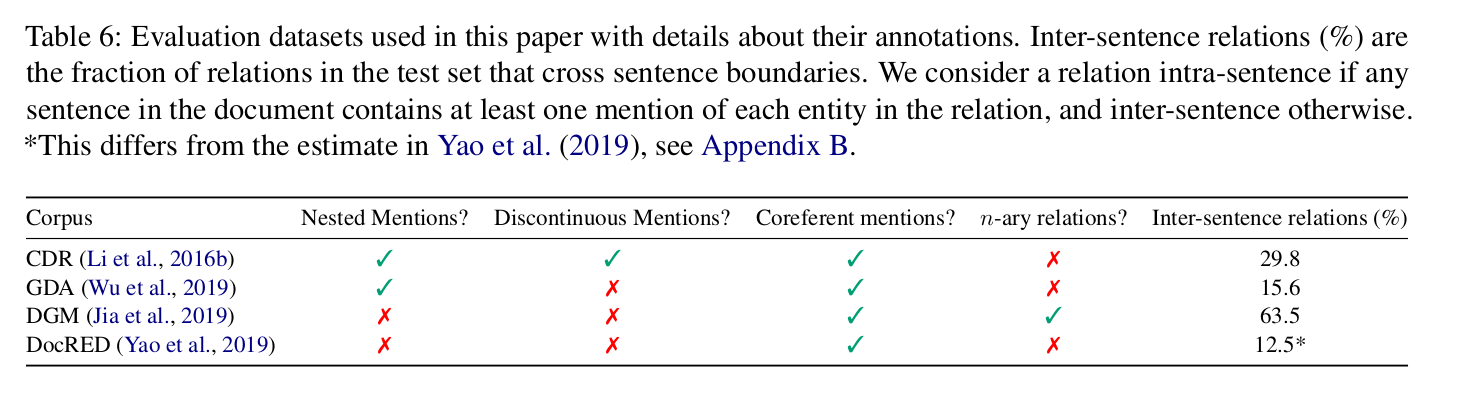
\includegraphics[width=1.0\textwidth,height=1.0\textheight,keepaspectratio]{datasetinfo} 
          \end{figure}
        \end{frame}
       
        
        \begin{frame}{Linearization Schema}
          \begin{figure}
          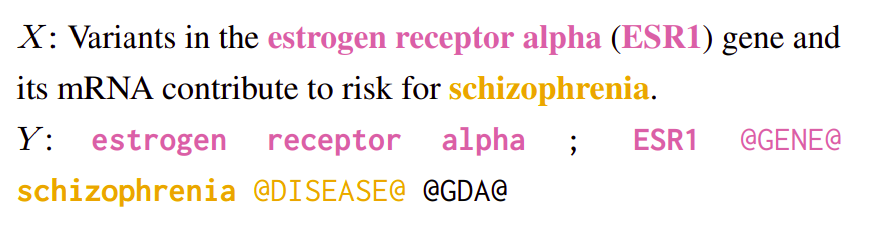
\includegraphics[width=0.7\textwidth,height=0.7\textheight,keepaspectratio]{linearization} 
          \end{figure}
          Full schema:

          
          \begin{adjustbox}{varwidth=\linewidth}%,scale=0.7}
            %% \begin{framed}
            %\centering
            \small\text{$<\textit{entity mention}_{1,1}>$ ; ... ; $<\textit{entity mention}_{1,n}>$ $@<\textit{entity type}_1> \dots$}


            \small\text{$<\textit{entity mention}_{m,1}>$ ; ... ; $<\textit{entity mention}_{m,k}>$ $@<\textit{entity type}_m>$}


            \small\text{$@<\textit{relation type}>$}
            \end{adjustbox}
        \end{frame}

        
        \begin{frame}{Model Structure}
          \begin{itemize}
          \item
            Seq2seq architectre.
          \item
            Decoder: Single-layer LSTM with randomly initialized weights.
          \item
            Encoder: PubMedBERT on DGM, GDA, and CDR.  $\text{BERT}_{\text{BASE}}$ for DocRED.
          \item
            Decoder generates special $@$START and $@$END tokens, along with entity and relation types.
          \item
            Decoder includes entity tokens in ouput via a including okens from the input text in output vocabulary\footnote{\textit{copy mechanism} in the authors' terms.}.
          \item
            6 head cross attention mechanism\footnote{https://vaclavkosar.com/ml/cross-attention-in-transformer-architecture} between encoder and decoder.
          \end{itemize}
        \end{frame}

        \begin{frame}{RE on Gold Entities with Entity Hinting}
          \begin{figure}
            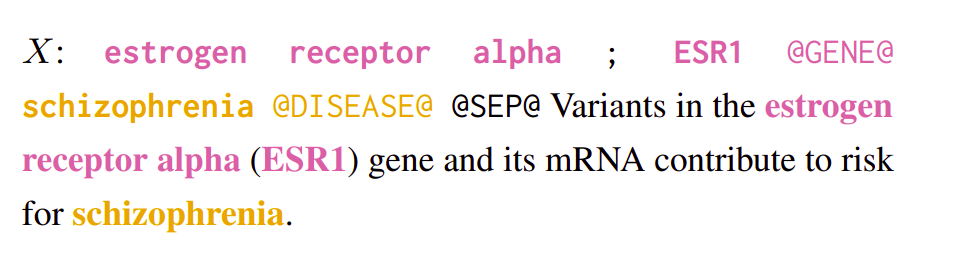
\includegraphics[width=0.7\textwidth,height=0.7\textheight,keepaspectratio]{entity_hint} 
          \end{figure}

          Full schema:

          \begin{adjustbox}{varwidth=\linewidth}%,scale=0.7}
            %% \begin{framed}
            %\centering
            \small\text{$<\textit{entity mention}_{1,1}>$ ; ... ; $<\textit{entity mention}_{1,n}>$ $@<\textit{entity type}_1> \dots$}

            
            \small\text{$<\textit{entity mention}_{m,1}>$ ; ... ; $<\textit{entity mention}_{m,k}>$ $@<\textit{entity type}_m> \ldots$}
            

            \small\text{$@\text{SEP}$ $<\textit{input text}>$}
          \end{adjustbox}
        \end{frame}

        
        
        \section{Results}

        
        
        \section{Analysis}


        \begin{frame}{$n$-ary Relations (DGM)}
          \begin{figure}
            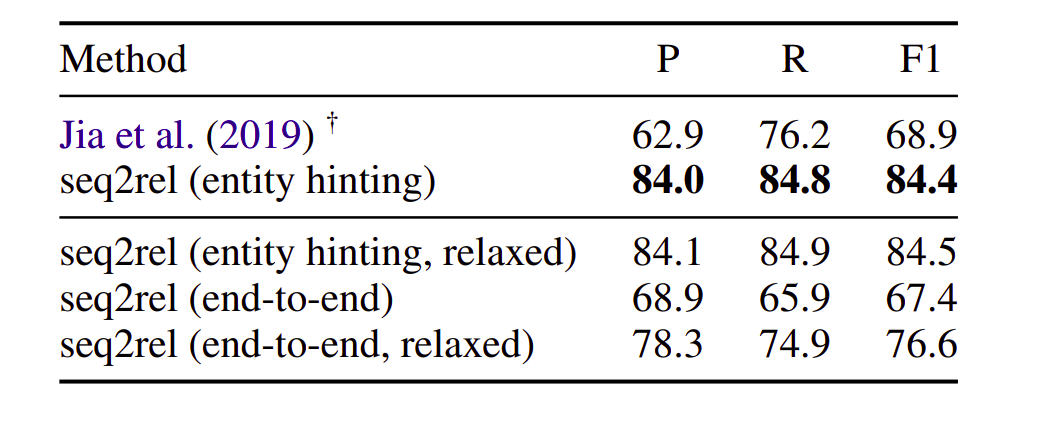
\includegraphics[width=0.7\textwidth,height=0.7\textheight,keepaspectratio]{DGM_n_ary_comparison} 
          \end{figure}
          DGM has ternary relations. Jia et al. (2019) uses multiscale architecture
          (uses multiple representations over different sizes of text spans and types of sub-relations).
          Both use gold entities (entity hinting in seq2rel case).
        \end{frame}

        \begin{frame}{RE with Gold Entities (CDR, GDA)}
          \begin{figure}
            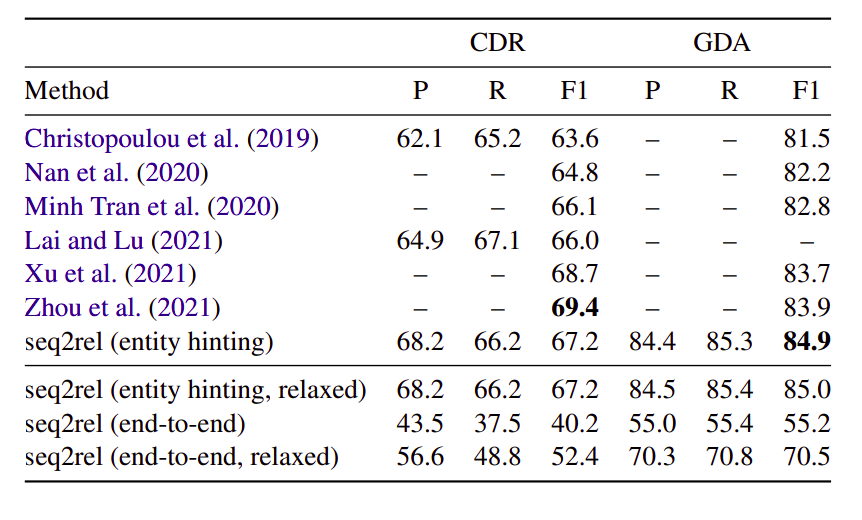
\includegraphics[width=0.7\textwidth,height=0.7\textheight,keepaspectratio]{CDR_GDA_gold_entities} 
          \end{figure}

          (Not enough room, full breakdown in paper appendix)
        \end{frame}

        \begin{frame}{End-to-end RE (DocRED)}
          \begin{figure}
            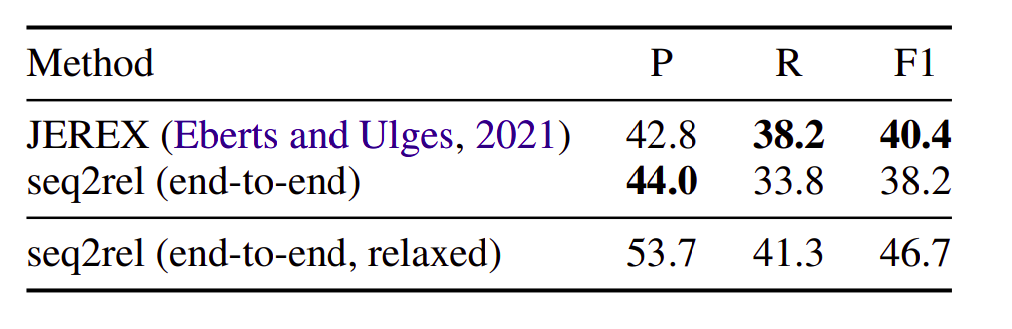
\includegraphics[width=0.7\textwidth,height=0.7\textheight,keepaspectratio]{DocRED_e2e_comparison} 
          \end{figure}

          Eberts and Ulges (2021) use JEREX.
          Extends BERT with four task-specific
          components that use BERTs outputs to per-
          form entity mention localization, coreference
          resolution, entity classification, and relation
          classification. They present two versions of
          their relation classifier, denoted “global re-
          lation classifier” (GRC) and “multi-instance
          relation classifier” (MRC). The authors compare against
          JEREX-MRC in DocRED end to end.
        \end{frame}


        \begin{frame}{End-to End RE Ablation (CDR, DocRED)}
          \begin{figure}
            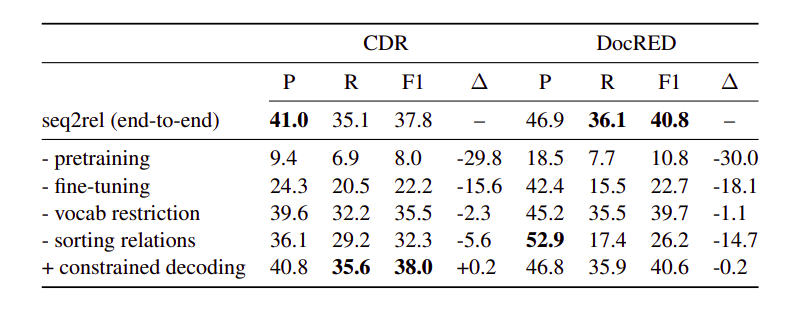
\includegraphics[width=0.7\textwidth,height=0.7\textheight,keepaspectratio]{ablation} 
          \end{figure}
          Fine-tuning here is fine-tuning of the encoder, decoder is fine-tuned regardless.  
        \end{frame}

        \begin{frame}{Training Set Size vs. Performance (CDR, GDA)}
          \begin{figure}
            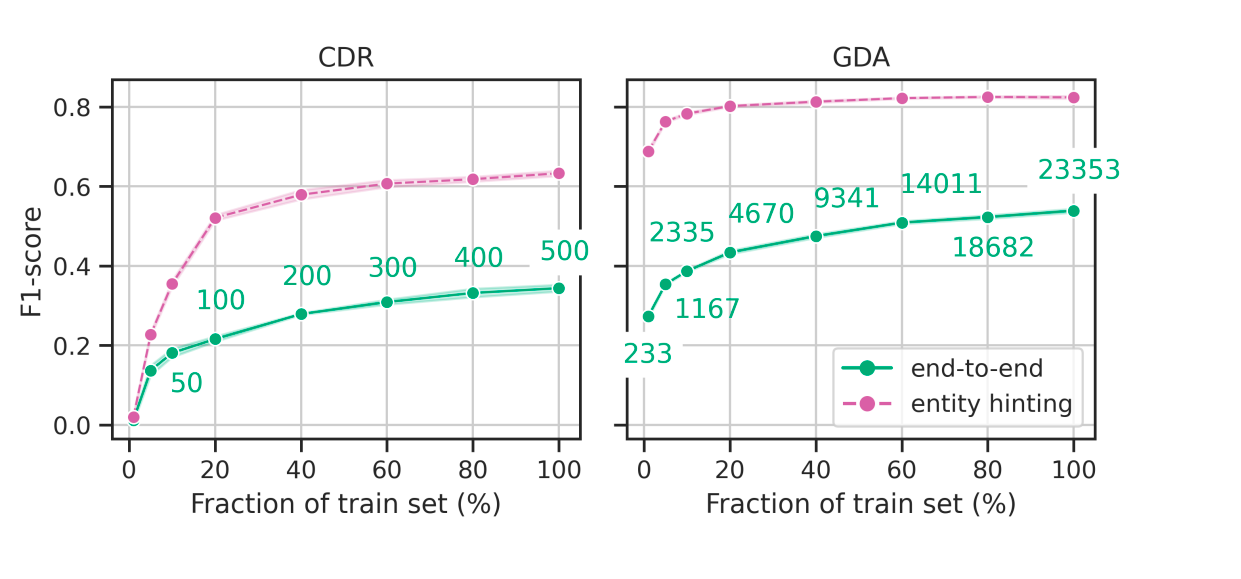
\includegraphics[width=0.7\textwidth,height=0.7\textheight,keepaspectratio]{training_set_size_plateau} 
          \end{figure}
        \end{frame}
        
        \section{Conclusion}

        \begin{frame}{Conclusion}


          See paper for bibliography.
        \end{frame}
      \end{document}
      
      
